\documentclass{tfg}

% The class already loads the packages used below for figures, tables,
% wrapped figures, landscape pages, captions, colors, hyperlinks, and
% bibliography. Add project-specific packages here only when needed.

\begin{document}

% ---------------------------------------------------------------------------
% Full-page cover image.
% Replace the PNG with your own A4 cover, keeping the same path if possible.
% ---------------------------------------------------------------------------
\coverpage{images/covers/cover.png}

% ---------------------------------------------------------------------------
% License page.
% Available license keys are the PNG filenames in images/licenses without .png:
% CC-0, CC-BY, CC-BYND, CC-BYNC, CC-BYNCND, CC-BYNCSA, CC-BYSA.
% ---------------------------------------------------------------------------
\begin{licensepage}{CC-BYSA}
  {YOUR PROJECT TITLE\\[0.5ex]
   A short subtitle that explains the scope of the work.}
  {Your Name}
  {Tutor Name}
  {\href{https://github.com/your-user/tfg-latex-template}{%
    
\includegraphics[width=0.58\linewidth]{images/others/codeQR.png}%
  }}
  {This template also demonstrates inline bibliographic entries such as
   \fullcite{templatepaper}.}
  {Madrid, Month 2026}
\end{licensepage}

\acknowledgmentpage{Use this page for short acknowledgements. The command
accepts one argument, so write the complete text between braces. You can still
use emphasis, links, citations, and the styled inline code command such as
\texttt{acknowledgmentpage}.}

\abstractpage{This abstract page is generated with \texttt{\string\abstractpage}.
The first argument is the abstract text. Use it to summarize the research
problem, the methodology, the main results, and the practical relevance of your
work in one or two compact paragraphs. The class uses custom fonts, spacing,
and page layout for this front-matter page.}
{LaTeX template, final degree project, reproducible writing}

\toc
\lof
\lot

\section{Template Overview}
\label{sec:overview}

This document is intentionally small, but it exercises the visual and structural
features provided by \texttt{tfg.cls}. Use it as a starting point by replacing
the sample text, figures, bibliography entries, and metadata with your own
project material.

The class configures the page geometry, headers, footers, fonts, section titles,
caption style, hyperlink colors, bibliography style, and several front-matter
commands. It also redefines \texttt{\string\texttt} so inline code has the same
visual treatment throughout the document.

\subsection{Headings, Links, and Code}
\label{subsec:headings}

Sections automatically begin on a new page and are rendered with the class
colors. Subsections receive a rule under the title, while subsubsections use an
italic style.

\subsubsection{A Third-Level Heading}
\label{subsubsec:third-level}

Internal links, citations, and web links use different colors. For example, see
\autoref{fig:single}, the table in \autoref{tab:class-features}, and the sample
source in \cite{templatedataset}. A web link can be written with
\href{https://www.overleaf.com/}{Overleaf}.

\begin{tcolorbox}[
  colback=rowshade,
  colframe=sectionblue,
  coltitle=white,
  title={Class color palette},
  sharp corners,
  boxrule=0.8pt
]
The class defines reusable colors such as \texttt{sectionblue},
\texttt{subsectiongray}, \texttt{rowshade}, \texttt{reflinkcolor},
\texttt{weblinkcolor}, and \texttt{intlinkcolor}. It also loads
\texttt{tcolorbox}, so you can build callouts with the same palette.
\end{tcolorbox}

\section{Figures and Visualizations}
\label{sec:figures}

The class loads \texttt{graphicx}, \texttt{caption}, \texttt{subcaption},
\texttt{wrapfig}, and \texttt{pdflscape}. The examples below show the most
common figure patterns for a TFG document.

\subsection{Single Figure}
\label{subsec:single-figure}

\begin{figure}[htbp]
  \centering
  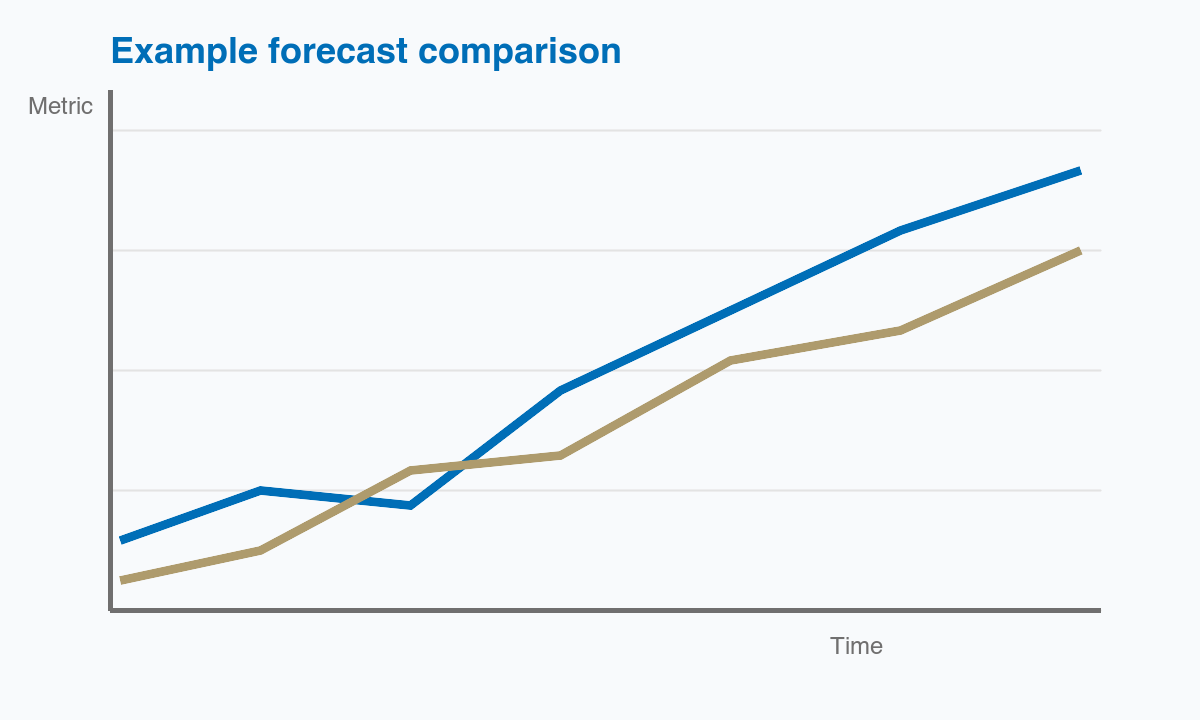
\includegraphics[width=0.82\linewidth]{images/plots/demo_chart.png}
  \captionsetup{width=0.82\linewidth}
  \caption[Short figure title for the list of figures]{A standard figure using
  the class caption format. The optional caption text appears in the list of
  figures, while this longer caption appears below the image.}
  \label{fig:single}
\end{figure}

\subsection{Subfigures}
\label{subsec:subfigures}

\begin{figure}[htbp]
  \centering
  \begin{subfigure}[t]{0.48\linewidth}
    \centering
    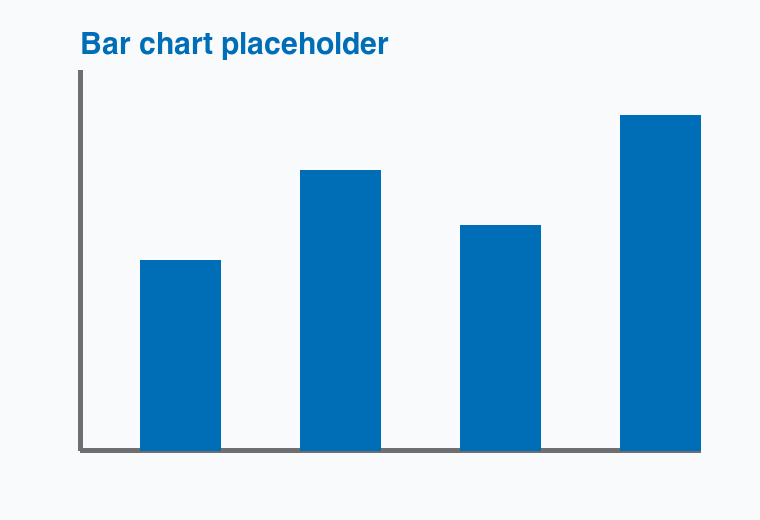
\includegraphics[width=\linewidth]{images/plots/demo_plot_a.png}
    \caption{First visualization.}
    \label{fig:sub-a}
  \end{subfigure}
  \hfill
  \begin{subfigure}[t]{0.48\linewidth}
    \centering
    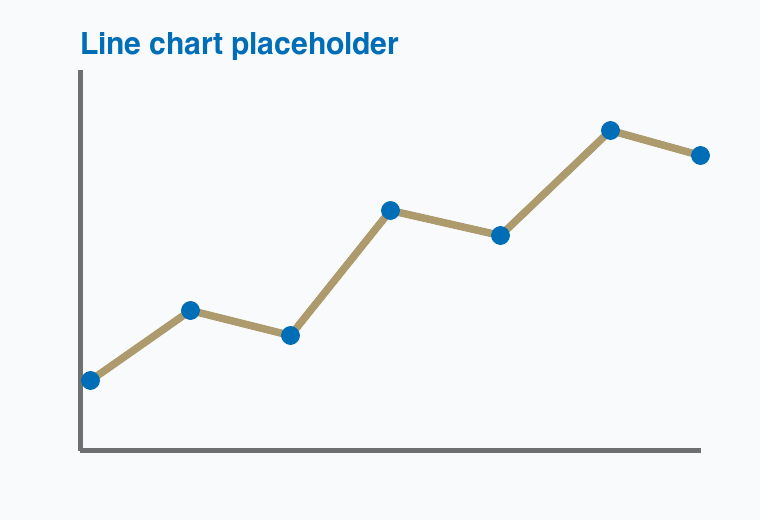
\includegraphics[width=\linewidth]{images/plots/demo_plot_b.png}
    \caption{Second visualization.}
    \label{fig:sub-b}
  \end{subfigure}
  \captionsetup{width=\linewidth}
  \caption[Subfigure layout]{A two-panel figure built with the
  \texttt{subcaption} package loaded by the class. You can reference panels as
  \autoref{fig:sub-a} and \autoref{fig:sub-b}.}
  \label{fig:subfigures}
\end{figure}

\subsection{Wrapped Figure}
\label{subsec:wrapped}

\begin{wrapfigure}[13]{r}{0.36\linewidth}
  \centering
  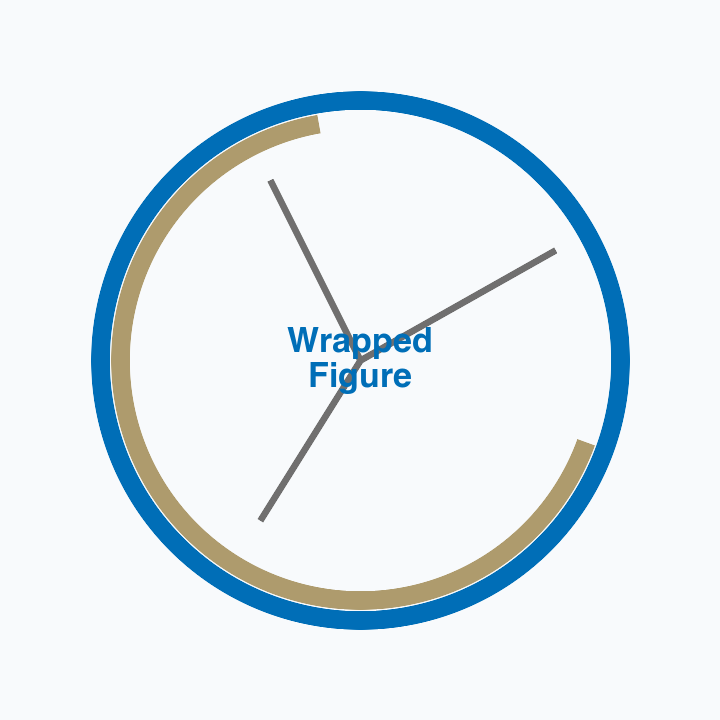
\includegraphics[width=\linewidth]{images/plots/demo_wrap.png}
  \captionsetup{width=\linewidth}
  \caption[Wrapped figure]{A wrapped figure beside paragraph text.}
  \label{fig:wrapped}
\end{wrapfigure}

Wrapped figures are useful when a compact visual supports the surrounding
discussion without needing a full-width float. Keep the wrapped figure close to
the paragraph that introduces it, and avoid placing it near section boundaries
where float placement becomes less predictable.

This paragraph adds enough text to show the wrapping behavior. In a thesis,
wrapped figures work best for diagrams, icons, or small plots that remain
legible at a reduced width. Larger visualizations should use a normal figure or
a landscape page instead.

\section{Tables}
\label{sec:tables}

The \texttt{mytable} environment is defined in \texttt{tfg.cls}. Its arguments
are placement, column specification, long caption, label, and an optional short
caption for the list of tables.

\renewcommand{\cellfont}{\footnotesize}
\begin{mytable}[htbp]
  {p{0.26\linewidth} p{0.34\linewidth} p{0.28\linewidth}}
  {Main custom commands and environments exposed by \texttt{tfg.cls}.}
  {tab:class-features}
  [Class features]
  \thead{Feature} & \thead{Purpose} & \thead{Typical use} \\
  \hline
  \texttt{\string\coverpage} & Creates a full-page image cover. &
  First page of the document. \\
  \texttt{licensepage} & Builds the metadata and Creative Commons page. &
  Title, author, tutor, QR, notes, and date. \\
  \texttt{\string\acknowledgmentpage} & Adds a styled acknowledgements page. &
  Optional front matter before the abstract. \\
  \texttt{\string\abstractpage} & Adds abstract text and keywords. &
  Summary and indexing terms. \\
  \texttt{\string\toc}, \texttt{\string\lof}, \texttt{\string\lot} &
  Prints styled contents, figures, and tables lists. &
  Front matter after the abstract. \\
  \texttt{mytable} & Applies row shading and caption formatting. &
  Reusable data tables. \\
\end{mytable}
\renewcommand{\cellfont}{\small}

\section{Wide Material}
\label{sec:wide}

Use the \texttt{landscape} environment when a wide diagram or table would be
too cramped on a portrait page.

\begin{landscape}
\begin{figure}[p]
  \centering
  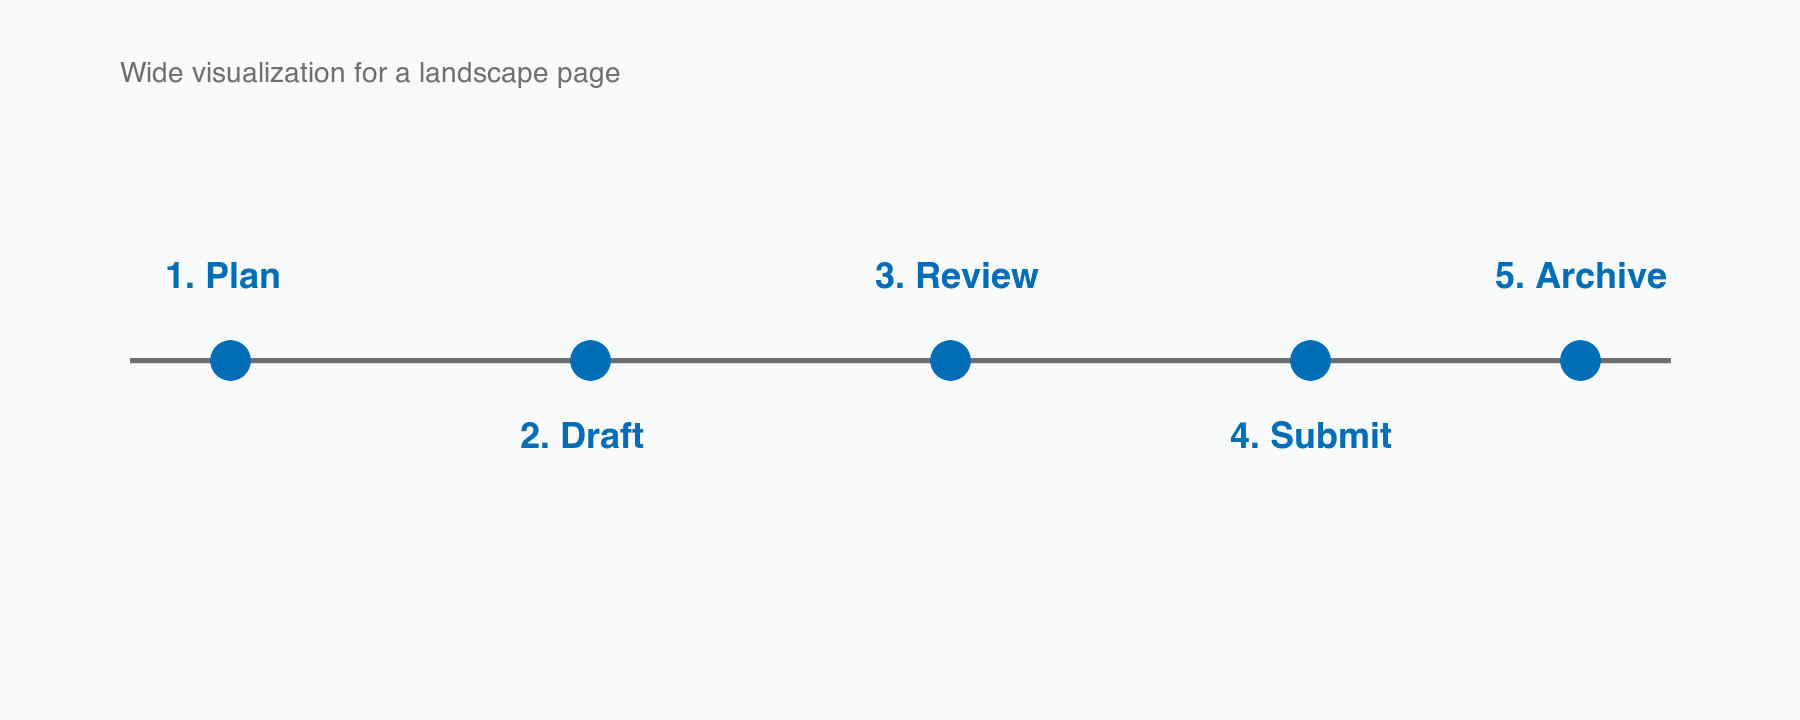
\includegraphics[width=0.92\linewidth]{images/plots/landscape_timeline.png}
  \captionsetup{width=0.9\linewidth}
  \caption[Landscape visualization]{A wide figure placed on a landscape page
  with the \texttt{pdflscape} package loaded by the class.}
  \label{fig:landscape}
\end{figure}
\end{landscape}

\section{Bibliography}
\label{sec:bibliography}

The class loads \texttt{biblatex} and expects a file named
\texttt{references.bib}. Cite sources normally with \texttt{\string\cite}, for
example \cite{templatepaper}, and print the bibliography with the custom
\texttt{mybigheading} heading:

\printbibliography[heading=mybigheading,title={References}]

\end{document}
